% !TeX spellcheck = en_US
\documentclass[french]{yLectureNote}

\title{Mécanique 2}
\subtitle{Chimie}
\author{Paulhenry Saux}
\date{\today}
\yLanguage{Français}

\professor{IHallery}%isabelle.hallery@univ-tlse3.fr
\usepackage{graphicx}%----pour mettre des images
\usepackage[utf8]{inputenc}%---encodage
\usepackage{geometry}%---pour modifier les tailles et mettre a4paper
%\usepackage{awesomebox}%---pour les boites d'exercices, de pbq et de croquis ---d\'esactiv\'e pour les TP de PC
\usepackage{tikz}%---pour deiffner + d\'ependance de chemfig
% \usepackage{tabularx}%---pour dimensionner automatiquement les tableaux avec variable X
\usepackage{awesomebox}%---Pour les boites info, danger et autres
\usepackage{menukeys}%---Pour deiffner les touches de Calculatrice
\usepackage{fancyhdr}%---pour les en-t\^ete personnalis\'ees
\usepackage{blindtext}%---pour les liens
\usepackage{hyperref}%---pour les liens (\`a mettre en dernier)
\usepackage{caption}%---pour la francisation de la l\'egende table vers Tableau
\usepackage{pifont}
\usepackage{array}%---pour les tableaux
\usepackage{lipsum}
\usepackage{yFlatTable}
\usepackage{multicol}
\newcommand{\Lim}[1]{\lim\limits_{\substack{#1}}\:}
\renewcommand{\vec}{\overrightarrow}
\newcommand{\N}[0]{\mathbb{N}}
\newcommand{\dd}{\mathrm{d}}
\newcommand{\norm}[1]{||\vec{#1}||}
\begin{document}
\setcounter{chapter}{2}
\chapter{Moment cinétique}
\section{Définition du moment cinétique d’un point matériel}
\subsection{ Moment cinétique par rapport à un point}
Soit un point O du référentiel R dans lequel on travaille.
Soit un point matériel M de masse m, de vitesse \()\vec{v}(M)\) et de quantité de mouvement
\(\vec{p} (M)\) par rapport au référentiel R.
Le moment cinétique de M par rapport à O dans le référentiel R est défini par le
vecteur\marginTips{Le fait que le mouvement d’un point matériel soit déterminé par la donnée d’un seul
vecteur implique qu’en mécanique du point, il n’est pas nécessaire d’utiliser en même
temps quantité de mouvement et moment cinétique. Le problème posé sera résolu par
la détermination de l’une ou de l’autre de ces quantités.
Là réside une différence essentielle avec la mécanique des solides où la détermination
des deux quantités que sont le moment cinétique et la quantité de mouvement sera
nécessaire.} :
\begin{definition}[Moment cinétique]
\[\vec{L_O} = \vec{OM} \wedge \vec{p} = \vec{OM} \wedge m \vec{v}\]
\end{definition}
\subsection{Propriétés}
\begin{itemize}
 \item \(\vec{OM} = 0 \Rightarrow \vec{L_O} = 0\)
 \item \(\vec{OM}, \vec{p}\) colinéaires \(\Rightarrow \vec{L_O} = 0\)
 \item \(\vec{L_O'} = \vec{O'O}\wedge \vec{p}+\vec{L_O}\) : Le moment cinétique dépend du point par rapport auquel on le détermine.
 \item \(\vec{O'O}//\vec{p} \Rightarrow \vec{L_O} = \vec{L_O'}\)
 \item \(\norm{L_O} = d\cdot p\) avec $d$ le bras de levier
 \item \(\vec{L_{tot}} = \sum \vec{L_i}\)
\end{itemize}
\subsection{Moment cinétique par rapport à un axe}
Soit un axe $\Delta$. On note O un point de cet axe et $\vec{u}$
 un vecteur unitaire directeur de
cet axe

On définit un moment cinétique $L_{\Delta}$ par rapport à l’axe $\Delta$ passant par O à l’aide de la
relation\marginWarning{Il est important de noter qu’un moment par rapport à un point est un vecteur tandis
qu’un moment par rapport à un axe est un scalaire.} : \[L_{\Delta} = \vec{L_O}\cdot \vec{u}\]
\section{Moment d'une force}
\begin{definition}
On appelle moment de la force f par rapport à un point O le vecteur :
\[\vec{M_O}(\vec{f}) = \vec{OM}\wedge \vec{f}\] avec $M$ le point matériel sur lequel s'applique la force.
\end{definition}


\warningInfo{Influence du point}{ Le moment des forces dépend du point où on le calcule et
on a  :
\[\vec{M_O'}(\vec{f}) = \vec{M_O}(\vec{f}) + \vec{O'O}\wedge \vec{f}\]
}
\checkInfo{Considérations pratiques}{
% Le produit vectiriuel en cartésien est celui habituel. Celui pour les coordonnées cylindriques donne \(\vec{L} = (-z\rho\dot{\varphi}), (\dot{\rho}z-\rho\dot{z}),(\dot{\rho}\ddot{\varphi})\)

On a, pour une force appliquée au point A \[\norm{M_O} = d \norm{f}\] avec d comme sur le schéma :

\includegraphics{bras}

% encart rose
}
\section{Théorème du moment cinétique}
\begin{theorem}[Théorème du moment cinétique]
La dérivée du moment cinétique du point M en un point fixe O par rapport au
temps est égale à la somme des moments des forces appliquées en M par rapport
au point fixe O.
 \[\frac{\dd \vec{L_O}}{\dd t} = \sum_i \vec{M_o}(\vec{f_i})\]
\end{theorem}
On n’appliquera le théorème du moment cinétique qu’en un point fixe O.
\begin{center}
\begin{tabular}{lll}
 Composante & Linéaire & Angulaire\\
Mouvement & \(\vec{p}\) & \(\vec{L}\)\\
Vitesse & \(\vec{v}\) & \(\vec{\omega}\)\\
Position & \(\vec{x}\) & \(\varphi\)\\
Force & \(\vec{F} = \frac{\dd \vec{p}}{\dd t }\) & \(\vec{M_O} = \frac{\dd \vec{L}}{\dd t}\)\\
\(E_c\) & \(\frac{mv^2}{2}\) & \(\frac{I\omega^2}{2}\)
\end{tabular}
\end{center}
\section{Exemple du pendule}
\includegraphics[scale=0.45]{pendule}

On s’intéresse au mouvement d’un pendule simple c’est-à-dire au mouvement d’une
masse ponctuelle m suspendue à l’extrémité d’un fil inextensible, de masse négligeable,
de longueur l dont l’autre extrémité est fixe.
À l’instant initial, le pendule est lâché sans vitesse

d'une position définie par l’angle $\theta_0$ entre la verticale
 descendante et la direction du pendule.

Bilan des forces :
\begin{itemize}
 \item Poids \(m\vec{g}\)
 \item Tension du fil \(\vec{R}\)
\end{itemize}
\subsection{Avec le moment cinétique}
 Avant d’appliquer le théorème du moment cinétique, on remarque que le mouvement est plan. On se place en coordonnées polaires

On calcule \(L_O\) en coordonnées cylindriques\marginCritical{On applique la m\^eme formule que pour les coordonnées cartésiennes car nous sommes toujours dans une BOND}
\[ \vec{L_O} = \vec{OM} \wedge m \vec{v} = ml^2\dot{\theta} \]

On sait aussi \[\frac{\dd \vec{L_O}}{\dd t} = \vec{M_O}(m\vec{g}) + \vec{M_O}(\vec{R})\]
 Finalement, \[\frac{\dd \vec{L_O}}{\dd t} = \frac{\dd(ml^2\dot{\theta})}{\dd t} = ml^2\ddot{\theta}\vec{e_z}\]

 Mais la tension est une force centrale, donc son moment de force est nul.

 De plus, \[\vec{M_O}(m\vec{g}) = -mgl\sin(\theta)\vec{e_z} \]

 En assemblant les résultats, on a \[
 ml^2\ddot{\theta} = -mgl\sin(\theta)\]
 qui donne une équation d'oscillateur harmonique en se rapprochant du point où \(\theta = 0\) \[\ddot{\theta} + \frac{g}{l}\sin(\theta) = 0\]

\end{document}
